%! Author = mariuszindel
%! Date = 25.01.21

\section{Block Code}


\subsection{Hammingdistanz $h$}
\begin{itemize}
    \item sicher korrigierbarer Fehler, wenn
    \item $m$ = Nachrichtenstellen
    \item $k$ = Kontrollstellen
\end{itemize}
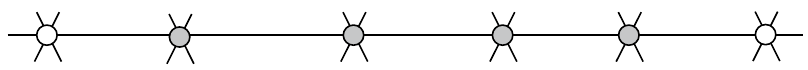
\includegraphics[width=\linewidth]{graphic/extern-reto/Hammingdistanz.png}
Jeder Knoten ist ein \textcolor{red}{Codewort}!\\
Sichere Erkennung von 4 Fehlern $\rightarrow$ Hammingdistanz = 5

\subsubsection{Anzahl aller Codeworte}
$n$ = Anzahl aller Spalten
\colorbox{lightlightgrey}{alle Codeworte = $2^n$}

\subsubsection{Anzahl gültige Codeworte}
$m$ = Anzahl Spalten der Prüfmatrix bis zur Einheitsmatrix\\
\colorbox{lightlightgrey}{gültige Codeworte = $2^m$}

\subsubsection{Sicher korrigierbarer Fehler}
$h$ \textcolor{red}{ungerade}: \colorbox{lightlightgrey}{$e = \frac{h - 1}{2}$}\hspace{3cm}\\
$h$ \textcolor{red}{gerade}: \colorbox{lightlightgrey}{$e = \frac{h - 2}{2}$}

\subsubsection{Dichtgepackt}
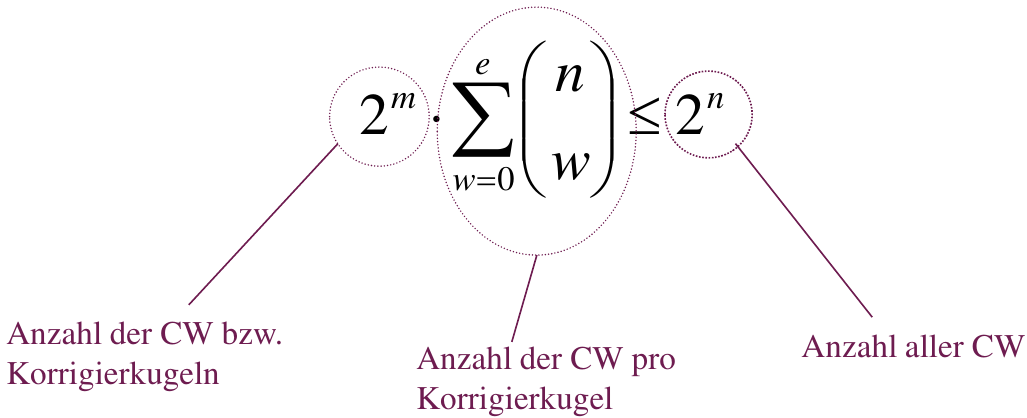
\includegraphics[width=\linewidth]{graphic/extern-reto/Dichtgepackt.png}\\
Wenn linker Teil = rechter Teil, Coderaum ist \textcolor{red}{Dichtgepackt}
\textit{Nspire: nCr(n,w)}

\subsubsection{Anzahl der Kontrollstellen $k$}
Bei Hammingcodes markiert die Einheitsmatrix in der Prüfmatrix die Anzahl der Kontrollstellen \colorbox{lightlightgrey}{$k = $ Spalten der Einheitsmatrix}

\subsubsection{Generatormatrix erstellen}
\begin{center}
    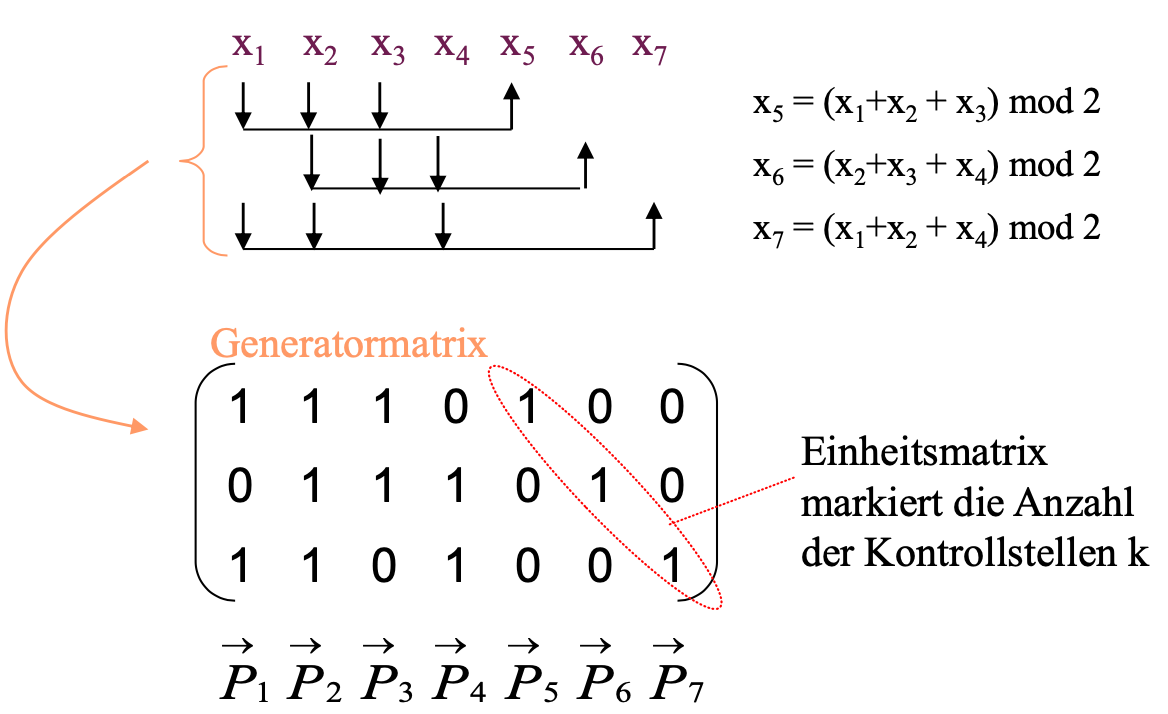
\includegraphics[width=\linewidth]{graphic/blockcode/generatormatrix.png}
\end{center}
\vspace{-8pt}



\subsubsection{Kontrollstellen ermitteln (Version 1)}
1. Grad bestimmen (xxxx), 2. Generator bestimmen(11101), 3. Wort bestimmen(100)\\
\vspace{-8pt}
\begin{center}
    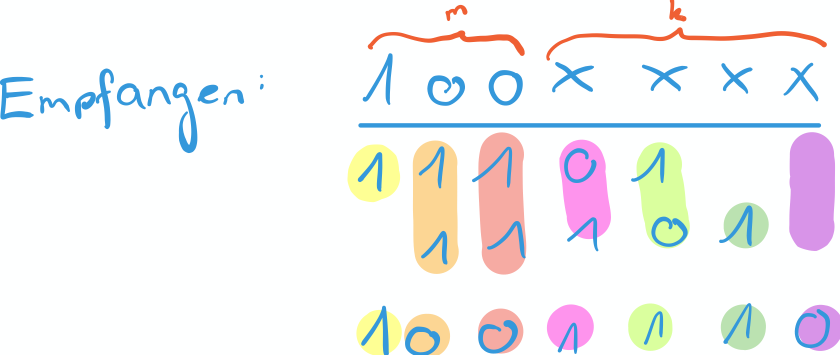
\includegraphics[scale=.3]{graphic/blockcode/kontrollstellen.png}
\end{center}
\vspace{-8pt}

\subsubsection{Kontrollstellen ermitteln (Version 2)}
1. Prüfmatrix gegeben, 2. Kontrollstellen k herauslesen (xxx), 3. Wort bestimmen(1000)\\
$(x_5 = x_1 + x_2 + x_3) mod 2$\\
$(x_6 = x_2 + x_3 + x_4) mod 2$\\
$(x_7 = x_1 + x_2 + x_4) mod 2$\\
Siehe auch Generatormatrix erstellen

\subsubsection{Fehlersyndrom bestimmen}
Bsp: $x_3$ ist gestört: Vektor $P_3$ aus Matrix lesen\\
Bsp: $x_3$ und $x_7$ ist gestört: Vektor $P_3 und P_7$ aus Matrix lesen und addieren mod 2\\




\subsection{Zyklischer Code}
Generatormatrix kann durch Generatorpolynom beschrieben werden\\
Das Codewortpolynom ist ohne Rest durch das Generatorpolynom teilbar (in mod-2-Rechnung)

\subsubsection{Grad bestimmen}
\colorbox{lightlightgrey}{$Grad = hoechste potenz$}

\subsubsection{Zyklische Abramson-Codes}
Diese werden gebildet durch die Multiplikation eines primitven Polynoms mit dem Term (1+x)
\colorbox{lightlightgrey}{$Abramson-Code: g(x)= p(x) (1+x)$}


\subsubsection{Gültige Codeworte mit Mehrfachaddition}
Grad des Generatorpolynoms entspricht Anzahl der Kontrollstellen k\\
$n = 2^k - 1$ und $n = m + k$
Generatorpolynom in Vektor umwandeln\\
%TODO


\subsubsection{gü̈ltige Codeworte mit Abramson}
$n = 2^{k-1} - 1$


\vfill
$$
\columnbreak